\documentclass[../manuale-utente.tex]{subfiles}

\begin{document}

\subsection{Scelta e inserimento di un file}
\label{subs:scelta-e-inserimento}
Una volta installata la training app è possibile scegliere un file \glossario{CSV}contenente i dati con cui si vuole compiere l'addestramento. Per caricare il file è sufficiente premere il pulsante sotto la scritta "CSV data file:"

\begin{figure}[h!]
  \begin{center}
    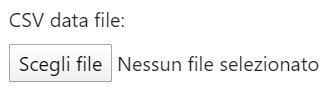
\includegraphics[width=4cm]{ScegliFile.png}\\
    \caption{Pulsante Scegli File}%
    \label{fig:scegli-file}
  \end{center}
\end{figure}
e selezionare il file che si vuole utilizzare. Il file CSV deve essere composto di valori separati da virgole. Qui di seguito è riportato un esempio:

\begin{figure}[h!]
  \begin{center}
    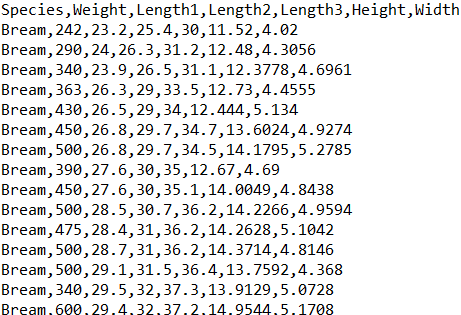
\includegraphics[width=10cm]{esempioCSV.png}\\
    \caption{Esempio file CSV}%
    \label{fig:esempioCSV}
  \end{center}
  \end{figure}

  È possibile, inoltre, inserire un file contenente un predittore allenato precedentemente.

\subsection{Scelta dell'algoritmo}
\label{subs:scelta-algoritmo}
Dopo aver caricato il file, è possibile scegliere l'algoritmo di machine learning con cui effettuare l'addestramento tra le opzioni disponibili:
\begin{itemize}
  \item RL (Regressione Lineare);
  \item SVM (Support Vector Machine).
\end{itemize}

\newpage
\subsection{Addestramento}
\label{subs:addestramento}

In seguito, sul lato destro della pagina comparirà il grafico contenente i dati presenti nel file. È possibile modificare le variabili degli assi utilizzando i menù a tendina presenti nella parte sottostante del grafico.\\
Nel caso venga selezionata la Regressione Lineare sarà possibile visualizzare la retta rappresentante il predittore ottenuto. Un esempio viene riportato di seguito:

\begin{figure}[h!]
  \begin{center}
    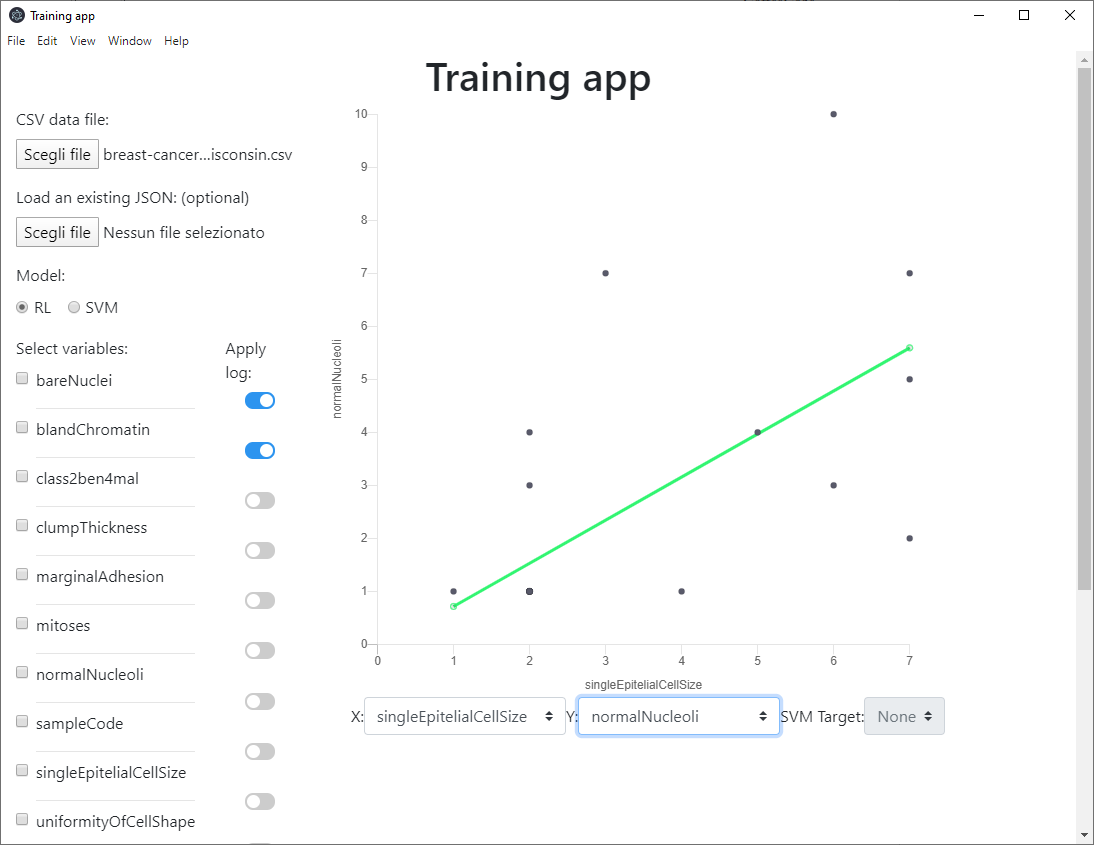
\includegraphics[width=16cm]{RL.png}\\
    \caption{Esempio RL}%
    \label{fig:RL}
  \end{center}
  \end{figure}


\newpage
Nel caso venga selezionata la Support Vector Machine sarà possibile visualizzare la posizione dei valori appartenenti alla stessa classe della variabile target. In seguito è riportato un esempio:

  \begin{figure}[h!]
    \begin{center}
      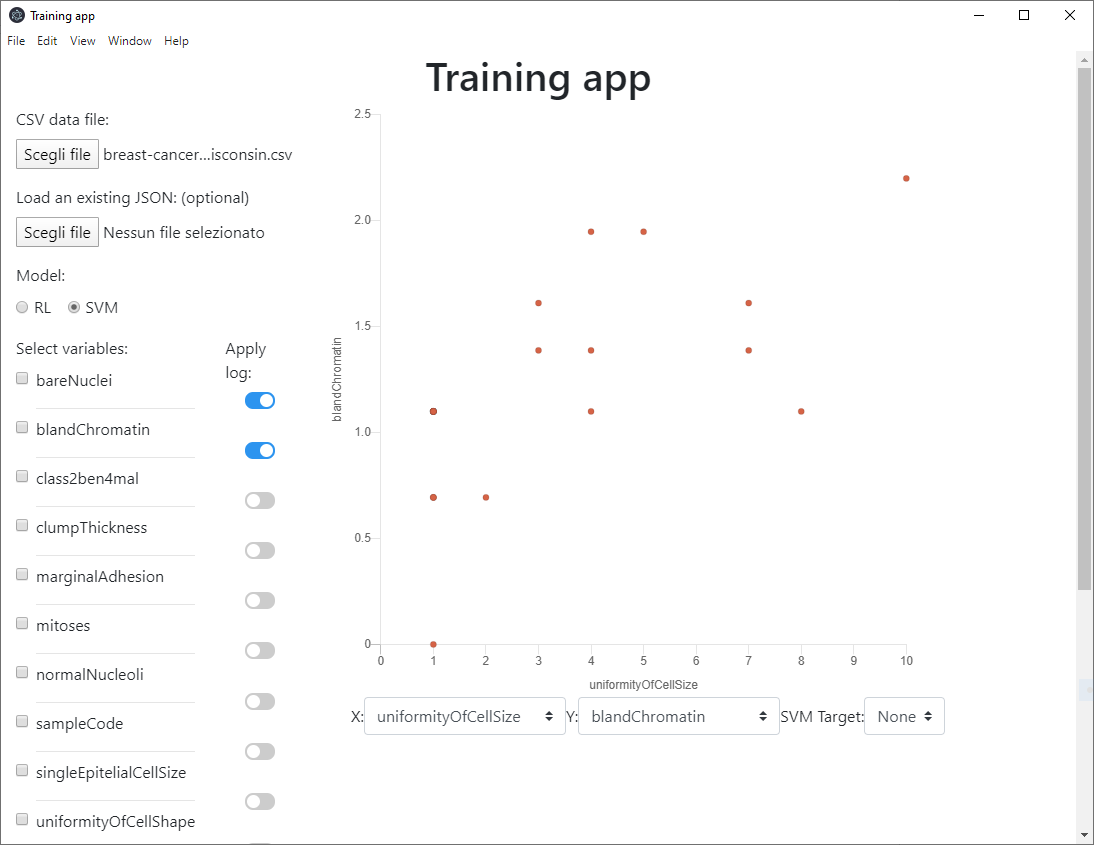
\includegraphics[width=16cm]{SVM.png}\\
      \caption{Esempio SVM}%
      \label{fig:SVM}
    \end{center}
    \end{figure}

\newpage
\subsection{Salvataggio del predittore}
\label{subs:salvataggio-del-predittore}
Premendo il pulsante "Submit" evidenziato in rosso

\begin{figure}[h!]
  \begin{center}
    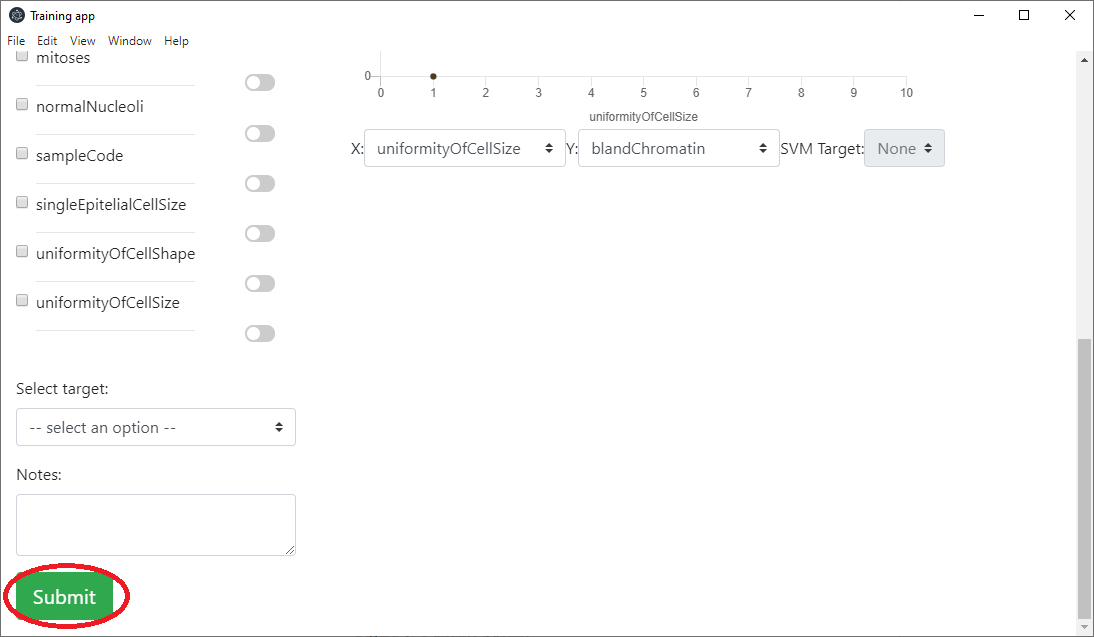
\includegraphics[width=16cm]{submit.png}\\
    \caption{Pulsante Submit}%
    \label{fig:pulsante-submit}
  \end{center}
\end{figure}

è possibile salvare il file in formato JSON contenente il predittore appena calcolato e al cui interno saranno presenti il tipo di algoritmo selezionato, i valori del coefficienti e il valore predetto della funzione.
A questo punto l'utente potrà compilare la form di sinistra indicando i dati che verranno usati come variabili ed il campo che verrà considerato come variabile obiettivo dall'algoritmo di machine learning. Infine, l'utente ha la possibilità di aggiungere alcune note in totale libertà per poter descrivere, ad esempio, i dati e le motivazione delle scelte.
\end{document}
